\documentclass[11pt]{article}    
\usepackage[a4paper,left=1in,right=1in,top=1in,bottom=1in]{geometry} 

\usepackage[english]{babel}
\usepackage[T1]{fontenc} 
\usepackage[utf8]{inputenc}
\usepackage{seqsplit}

\renewcommand{\familydefault}{\sfdefault} 
\usepackage{setspace}  \singlespacing  
\usepackage{graphicx}        
\usepackage[absolute]{textpos}
\usepackage{xcolor}
\usepackage{fontawesome5}
\usepackage{multirow}
\usepackage{hyperref}
\hypersetup{
    colorlinks,
    linkcolor={red!50!black},
    citecolor={blue!50!black},
    urlcolor={blue}
}

% Additional packages for the content
\usepackage{float}
\usepackage{subfig,wrapfig}
\usepackage{amsmath,amsfonts,amsthm,amssymb}
\usepackage{fancyhdr,fancybox,color}
\usepackage{enumerate}
\usepackage[amssymb]{SIunits}
\definecolor{MyBlue}{rgb}{0,0.3,0.6}
\usepackage[all]{hypcap}
\usepackage{csquotes}
\usepackage[url=false,
backend=bibtex,
style=authoryear-comp,
doi=true,
isbn=true,
backref=false,
dashed=false,
maxcitenames=2,
maxbibnames=99,
natbib=true]{biblatex}
\DeclareNameAlias{author}{family-given}
\renewbibmacro{in:}{}

\addbibresource{../_logosAndRef/references.bib}
\nonfrenchspacing

% Configurable separation between header and body
\newlength{\headertobodysep}
\setlength{\headertobodysep}{1cm}

% Header with logos and contact information
\begin{document}
\thispagestyle{empty}

% Lean header with aligned elements
\textblockorigin{0pt}{0pt}

% Durham logo on the left
\begin{textblock*}{5cm}(0.5cm,1cm)
    
\includegraphics[height=2cm]{../_logosAndRef/Durham-University.pdf}
\end{textblock*}

% Contact information in the center - vertically centered with logos
\begin{textblock*}{9cm}(6cm,1.5cm)
    \centering
    {\large \textbf{Playing ping-pong with liquid droplets | CoMPhy Lab}}\\[0.2em]
    Department of Physics, Durham University\\[0.3em]
    \href{https://comphy-lab.org}{comphy-lab.org}
\end{textblock*}

% CoMPhy logo aligned with right margin
\begin{textblock*}{5cm}(15.5cm,1cm) % exactly 1 cm away from the right edge
    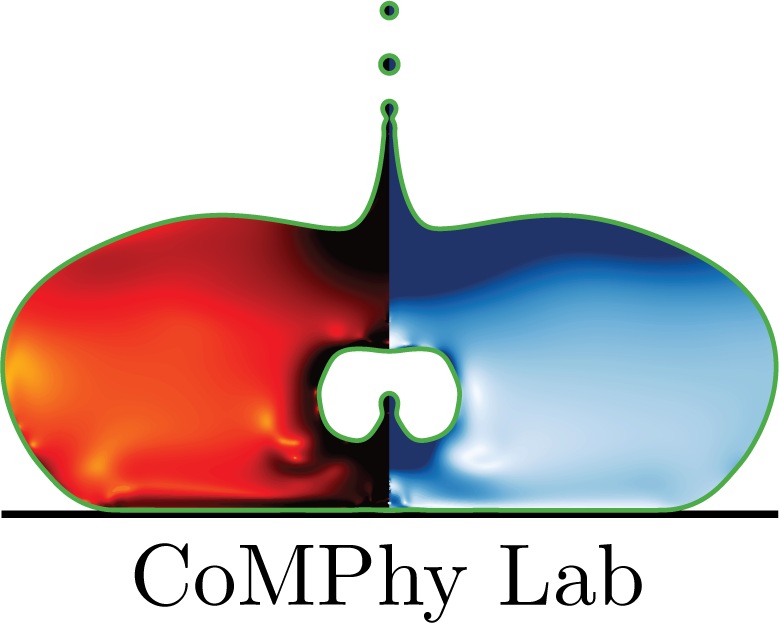
\includegraphics[height=2cm]{../_logosAndRef/CoMPhy-Lab.png}
\end{textblock*}

% Reset to normal text flow after header
\vspace*{\headertobodysep}

\begin{center}
    \begin{LARGE}
     Playing ping-pong with liquid droplets
    \end{LARGE}
\end{center}

\section*{Description}

Recently, during one of his trips to the International Space Station, astronaut Scott Kelly demonstrated that one could play ping-pong in space using water drops (\href{https://www.youtube.com/watch?v=TLbhrMCM4_0}{link here}). This demonstration follows from a long history of research on bouncing drops on superhydrophobic surfaces (see the discussions related to bouncing off superhydrophobic surfaces in \citet{josserand2016drop, VatsalThesis}).\\

In this study, we would like to further our understanding of this process of bouncing droplets \citep{zhang2022impact, vatsalInProgress, sanjay2022drop}. A typical sequence of events is shown in Figure~\ref{Figure::Typical}. In our simulation, we will use an in-house developed read-to-use code to solve the problem of the liquid drop impact on non-wetting substrates. We will focus on the hydrodynamics of the process. 

\begin{figure}[H]
\begin{center}
 \includegraphics[width=\textwidth]{SingularJets.eps}
 \caption{A typical simulation of a drop bouncing off a superhydrophobic substrate: (a) impacting drop with a constant velocity, (b) inertial shock as the drop hits the substrate, (c, d) the drop spreads on the substrate forming pyramidal shape owing to the propagating capillary waves on the surface of the drop \citep{renardy2003pyramidal, zhang2022impact}, (e) converging capillary waves create an air cavity, and (f, g) collapse of the air cavity entrains a bubble inside the drop and forms a thin and fast Worthington jet reminiscent of the hydrodynamic singularity \citep{Bartolo2006Singular}.}
 \label{Figure::Typical}
\end{center}

\end{figure}
\section*{What will you do and what will you learn?}
In the Physics of Fluids group, we are looking for enthusiastic students to work on this topic.
\begin{enumerate}
\itemsep0em
\item You will learn about fundamental fluid dynamics.
\item You will get hands-on experience with Computational Fluid Dynamics (CFD).
\item You will learn how to do basic and advanced data analysis.
\item You will learn how to document and publish ready-to-use codes and share them with the community, similar to \citet{basiliskVatsal, basiliskVatsalDropFilm, basiliskVatsalViscousBouncing}. 
\item As a part of the \href{https://comphy-lab.org}{CoMPhy lab}, you will learn and adapt open-source coding principles. 
\end{enumerate}

As a part of your bachelor's/master's assignment, we would like you to explore the field and come up with exciting avenues. To get you started, here is a list of open questions:

\begin{enumerate}
 \item How much force does the drop apply on the substrate? How does this force depend on the properties of the drop and the substrate properties?
 \item In the limit of zero impact velocities, capillarity dominates over the inertia of the impacting drop. We would like to understand the dynamics (including normal contact force and coefficient of restitution) in this limit of capillary oscillations. 
 \item One of the critical features is this process of impacting drops is viscous dissipation. For example, the dissipation occurs in the boundary layer inside the drop attached to the drop-air interface in the limit of zero viscosities. Surprisingly, the viscous dissipation does not vanish even in the vanishing viscosity limit, a behavior attributed to the dissipation anomaly. We would like to understand the role of viscous dissipation in this process. 
 \item Hydrodynamic singularities in drop impact. See: \citet{mandre2012mechanism} for impact time singularity and \citet{Bartolo2006Singular, sanjay_lohse_jalaal_2021, zhang2022impact} for singular jets. 
\end{enumerate} 

If you have any questions, feel free to contact us \href{mailto:vatsal.sanjay@comphy-lab.org}{vatsal.sanjay@comphy-lab.org}/\href{mailto:vatsal.sanjay@durham.ac.uk}{vatsal.sanjay@durham.ac.uk} or drop by Ph255 at the Department of Physics at Durham University.
\begin{center}
\begin{tabular}{|l|l|l|}
\hline \textbf{Collaborators} & \textbf{E-mail} & \textbf{Based at} \\
\hline \multirow{2}{*}{Dr. Vatsal Sanjay} & \href{mailto:vatsal.sanjay@comphy-lab.org}{vatsal.sanjay@comphy-lab.org} & \multirow{2}{*}{Ph255 (Rochester building)} \\
& \href{mailto:vatsal.sanjay@durham.ac.uk}{vatsal.sanjay@durham.ac.uk} & \\
\hline Ayush Dixit & \href{mailto:a.k.dixit@utwente.nl}{a.k.dixit@utwente.nl} & Univ. Twente \\
\hline Prof. Dr. Detlef Lohse & \href{mailto:d.lohse@utwente.nl}{d.lohse@utwente.nl} & Univ. Twente  \\
\hline
\end{tabular}
\end{center}

\vspace{1em}
\noindent\textit{Last updated: \today}

\printbibliography
\end{document}
\end{center}

\vspace{1em}
\noindent\textit{Last updated: \today}

\printbibliography

\end{document}
|||||||
=======
\documentclass[11pt]{article}    
\usepackage[a4paper,left=1in,right=1in,top=1in,bottom=1in]{geometry} 

\usepackage[english]{babel}
\usepackage[T1]{fontenc} 
\usepackage[utf8]{inputenc}
\usepackage{seqsplit}

\renewcommand{\familydefault}{\sfdefault} 
\usepackage{setspace}  \singlespacing  
\usepackage{graphicx}        
\usepackage[absolute]{textpos}
\usepackage{xcolor}
\usepackage{fontawesome5}
\usepackage{multirow}
\usepackage{hyperref}
\hypersetup{
    colorlinks,
    linkcolor={red!50!black},
    citecolor={blue!50!black},
    urlcolor={blue}
}

% Additional packages for the content
\usepackage{float}
\usepackage{subfig,wrapfig}
\usepackage{amsmath,amsfonts,amsthm,amssymb}
\usepackage{fancyhdr,fancybox,color}
\usepackage{enumerate}
\usepackage[amssymb]{SIunits}
\definecolor{MyBlue}{rgb}{0,0.3,0.6}
\usepackage[all]{hypcap}
\usepackage{csquotes}
\usepackage[url=false,
backend=bibtex,
style=authoryear-comp,
doi=true,
isbn=true,
backref=false,
dashed=false,
maxcitenames=2,
maxbibnames=99,
natbib=true]{biblatex}
\DeclareNameAlias{author}{family-given}
\renewbibmacro{in:}{}
\addbibresource{../_logosAndRef/references.bib}
\nonfrenchspacing

% Configurable separation between header and body
\newlength{\headertobodysep}
\setlength{\headertobodysep}{1cm}

% Header with logos and contact information
\begin{document}
\thispagestyle{empty}

% Lean header with aligned elements
\textblockorigin{0pt}{0pt}

% Durham logo on the left
\begin{textblock*}{5cm}(0.5cm,1cm)
    
\includegraphics[height=2cm]{../_logosAndRef/Durham-University.pdf}
\end{textblock*}

% Contact information in the center - vertically centered with logos
\begin{textblock*}{9cm}(6cm,1.5cm)
    \centering
    {\large \textbf{Playing ping-pong with liquid droplets | CoMPhy Lab}}\\[0.2em]
    Department of Physics, Durham University\\[0.3em]
    \href{https://comphy-lab.org}{comphy-lab.org}
\end{textblock*}

% CoMPhy logo aligned with right margin
\begin{textblock*}{5cm}(15.5cm,1cm) % exactly 1 cm away from the right edge
    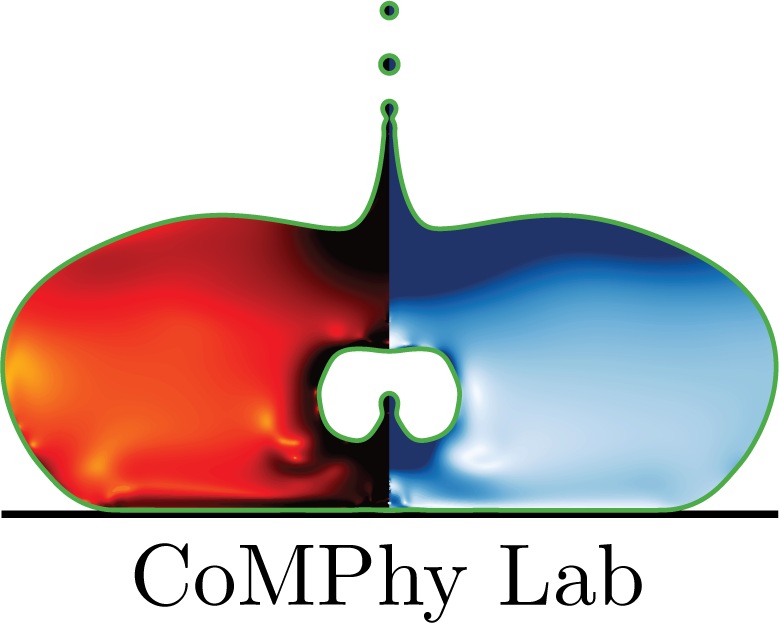
\includegraphics[height=2cm]{../_logosAndRef/CoMPhy-Lab.png}
\end{textblock*}

% Reset to normal text flow after header
\vspace*{\headertobodysep}

\begin{center}
    \begin{LARGE}
     Playing ping-pong with liquid droplets
    \end{LARGE}
\end{center}

\section*{Description}

Recently, during one of his trips to the International Space Station, astronaut Scott Kelly demonstrated that one could play ping-pong in space using water drops (\href{https://www.youtube.com/watch?v=TLbhrMCM4_0}{link here}). This demonstration follows from a long history of research on bouncing drops on superhydrophobic surfaces (see the discussions related to bouncing off superhydrophobic surfaces in \citet{josserand2016drop, VatsalThesis}).\\

In this study, we would like to further our understanding of this process of bouncing droplets \citep{zhang2022impact, vatsalInProgress, sanjay2022drop}. A typical sequence of events is shown in Figure~\ref{Figure::Typical}. In our simulation, we will use an in-house developed read-to-use code to solve the problem of the liquid drop impact on non-wetting substrates. We will focus on the hydrodynamics of the process. 

\begin{figure}[H]
\begin{center}
 \includegraphics[width=\textwidth]{SingularJets.eps}
 \caption{A typical simulation of a drop bouncing off a superhydrophobic substrate: (a) impacting drop with a constant velocity, (b) inertial shock as the drop hits the substrate, (c, d) the drop spreads on the substrate forming pyramidal shape owing to the propagating capillary waves on the surface of the drop \citep{renardy2003pyramidal, zhang2022impact}, (e) converging capillary waves create an air cavity, and (f, g) collapse of the air cavity entrains a bubble inside the drop and forms a thin and fast Worthington jet reminiscent of the hydrodynamic singularity \citep{Bartolo2006Singular}.}
 \label{Figure::Typical}
\end{center}

\end{figure}
\section*{What will you do and what will you learn?}
In the Physics of Fluids group, we are looking for enthusiastic students to work on this topic.
\begin{enumerate}
\itemsep0em
\item You will learn about fundamental fluid dynamics.
\item You will get hands-on experience with Computational Fluid Dynamics (CFD).
\item You will learn how to do basic and advanced data analysis.
\item You will learn how to document and publish ready-to-use codes and share them with the community, similar to \citet{basiliskVatsal, basiliskVatsalDropFilm, basiliskVatsalViscousBouncing}. 
\item As a part of the \href{https://comphy-lab.org}{CoMPhy lab}, you will learn and adapt open-source coding principles. 
\end{enumerate}

As a part of your bachelor's/master's assignment, we would like you to explore the field and come up with exciting avenues. To get you started, here is a list of open questions:

\begin{enumerate}
 \item How much force does the drop apply on the substrate? How does this force depend on the properties of the drop and the substrate properties?
 \item In the limit of zero impact velocities, capillarity dominates over the inertia of the impacting drop. We would like to understand the dynamics (including normal contact force and coefficient of restitution) in this limit of capillary oscillations. 
 \item One of the critical features is this process of impacting drops is viscous dissipation. For example, the dissipation occurs in the boundary layer inside the drop attached to the drop-air interface in the limit of zero viscosities. Surprisingly, the viscous dissipation does not vanish even in the vanishing viscosity limit, a behavior attributed to the dissipation anomaly. We would like to understand the role of viscous dissipation in this process. 
 \item Hydrodynamic singularities in drop impact. See: \citet{mandre2012mechanism} for impact time singularity and \citet{Bartolo2006Singular, sanjay_lohse_jalaal_2021, zhang2022impact} for singular jets. 
\end{enumerate} 

If you have any questions, feel free to contact us \href{mailto:vatsal.sanjay@comphy-lab.org}{vatsal.sanjay@comphy-lab.org}/\href{mailto:vatsal.sanjay@durham.ac.uk}{vatsal.sanjay@durham.ac.uk} or drop by Ph255 at the Department of Physics at Durham University.
\begin{center}
\begin{tabular}{|l|l|l|}
\hline \textbf{Collaborators} & \textbf{E-mail} & \textbf{Based at} \\
\hline \multirow{2}{*}{Dr. Vatsal Sanjay} & \href{mailto:vatsal.sanjay@comphy-lab.org}{vatsal.sanjay@comphy-lab.org} & \multirow{2}{*}{Ph255 (Rochester building)} \\
& \href{mailto:vatsal.sanjay@durham.ac.uk}{vatsal.sanjay@durham.ac.uk} & \\
\hline Ayush Dixit & \href{mailto:a.k.dixit@utwente.nl}{a.k.dixit@utwente.nl} & Univ. Twente \\
\hline Prof. Dr. Detlef Lohse & \href{mailto:d.lohse@utwente.nl}{d.lohse@utwente.nl} & Univ. Twente  \\
\hline
\end{tabular}
\end{center}

\vspace{1em}
\noindent\textit{Last updated: \today}

\printbibliography

\end{document}
